\section{Mô tả tính năng của phần mềm}
Đồ án Game Caro cung cấp một phần mềm mô phỏng môn thể thao cờ Caro, với tính năng 2 người chơi. Phần mềm cung cấp đầy đủ các tính năng cơ bản của một game Caro như cho phép nhập tên người chơi, tính năng thay đổi kích cỡ bảng cờ, tính năng xác định thắng thua, tính năng chọn bao nhiêu quân cờ liên tiếp để xác định thắng thua, tính năng điều chỉnh âm lượng,...

\subsection{Màn hình khởi động của game}
Hình sau đây là màn hình khởi động của game, với các nút cho phép người dùng lựa chọn các chức năng của trò chơi, theo thứ tự từ trên xuống dưới: chế độ 2 người chơi(\verb|PvP|), lựa chọn tiếp tục chơi (\verb|Continue|), cài đặt (\verb|Settings|), lựa chọn thoát (\verb|Quit|).

\begin{figure}[H]
\centering{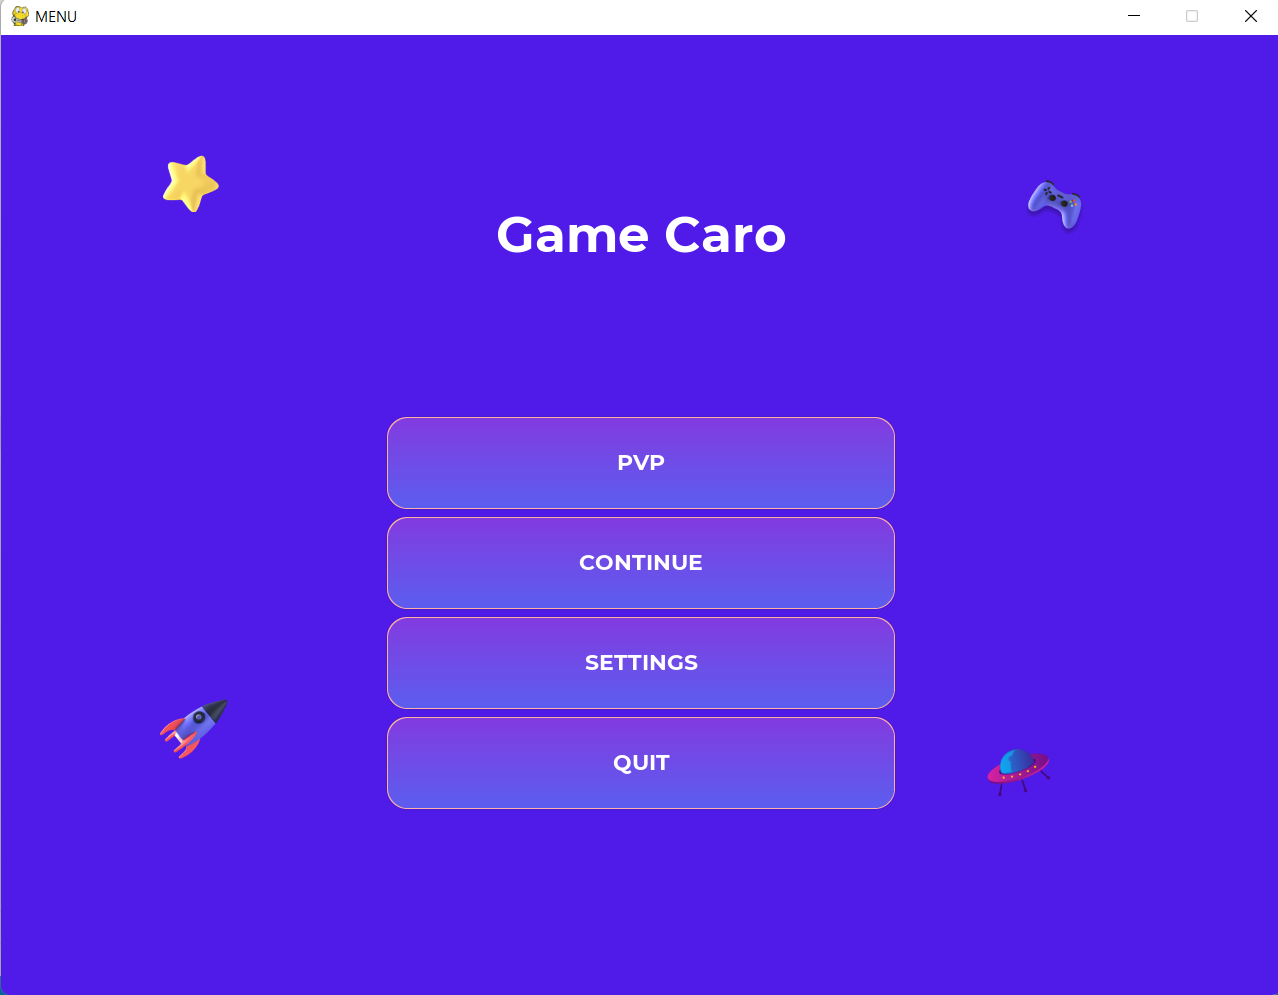
\includegraphics[scale=0.5]{images/menuscreen.png}}
\caption{Màn hình khởi động của game}
\end{figure}
\subsection{Lựa chọn Continue}
Khi người chơi nhấn chọn nút \verb|Continue| trên màn hình khởi động game, phần mềm sẽ chuyển đến màn hình game của ván game gần nhất trước đó nếu ván chưa kết thúc. Mặt khác, nếu ván game đã kết thúc, ô cửa sổ \verb|No game available| như hình bên dưới sẽ hiện lên, nhằm thông báo với người chơi rằng \textit{Không có dữ liệu của ván game cũ, hãy bắt đầu ván game mới}.
\begin{figure}[H]
\centering{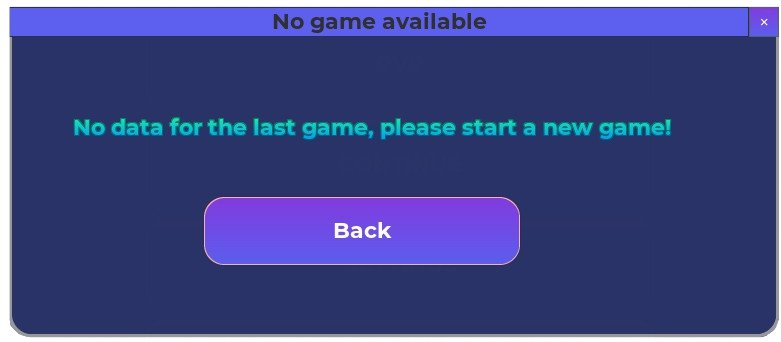
\includegraphics[scale=0.5]{images/continue.png}}
\caption{Cửa sổ No game available}
\end{figure}
\subsection{Lựa chọn cài đặt}
Vì có một số cài đặt (ví dụ: thay đổi kích cỡ bàn cờ) có thể làm ghi đè và xóa dữ liệu của ván game trước, nên khi bấm vào nút \verb|Settings| đầu tiên ta sẽ nhận được cửa sổ thông báo về việc sẽ mất dữ liệu khi thay đổi cài đặt, được trình bày ở hình bên dưới.
\begin{figure}[H]
\centering{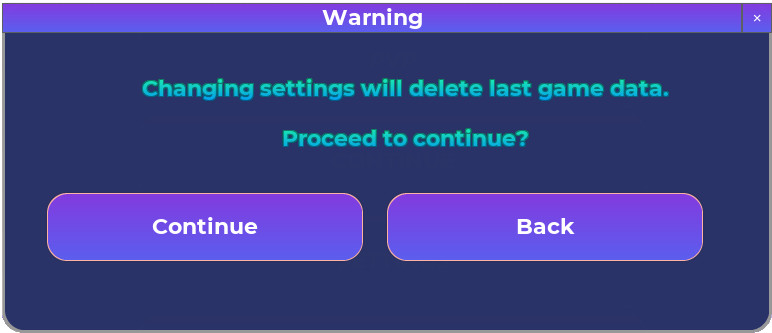
\includegraphics[scale=0.5]{images/setting.png}}
\caption{Cửa sổ cảnh báo mất dữ liệu}
\end{figure}

Nếu muốn quay lại màn hình khởi động của game, nhấn \verb|Back|. Ngược lại, nếu ta lựa chọn tiếp tục (tức ấn nút \verb|Continue|), cửa sổ \verb|Setting| sẽ hiện ra như hình bên dưới.
\begin{figure}[H]
\centering{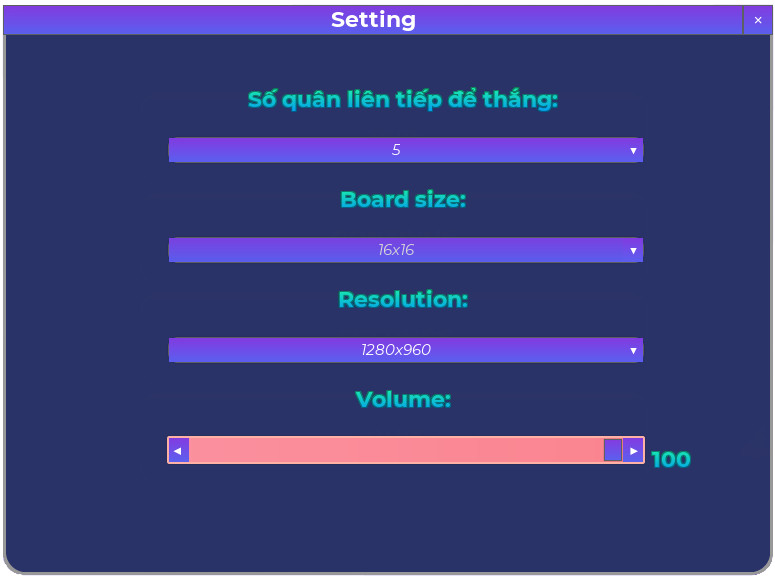
\includegraphics[scale=0.5]{images/setting1.png}}
\caption{Cửa sổ Setting}
\end{figure}

Ở ô cửa sổ này, người chơi được lựa chọn các tính năng hỗ trợ cho game. Đầu tiền là tính năng chọn số quân liên tiếp để thắng:\\
\begin{figure}[H]
\centering{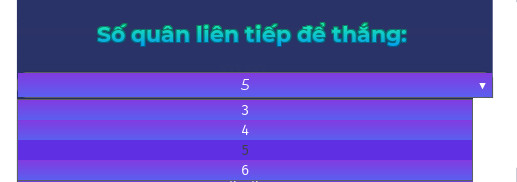
\includegraphics[scale=0.75]{images/setting2.png}}
\caption{Chọn số quân liên tiếp để thắng}
\end{figure}
Hình dưới đây minh họa cho tính năng chọn kích cỡ bàn cờ tương ứng với số quân cờ liên tiếp để thắng là 5:\\
\begin{figure}[H]
\centering{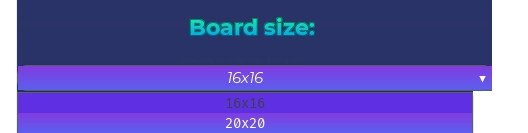
\includegraphics[scale=0.5]{images/boardsize.png}}
\caption{Chọn kích cỡ bảng cờ}
\end{figure}
Tính năng điều chỉnh âm lượng với thanh âm lượng chạy từ 0 đến 100:\\
\begin{figure}[H]
\centering{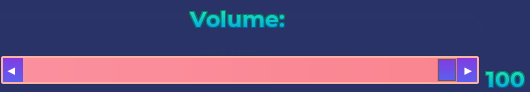
\includegraphics[scale=0.75]{images/volume.png}}
\caption{Điều chỉnh âm lượng}
\end{figure}
\subsection{Màn hình đặt tên người chơi}
Hình sau là màn hình đặt tên người chơi khi chọn chế độ chơi người với người (\verb|PvP|), ở đây ta có thể nhấn \verb|Back| để quay lại màn hình khởi động hoặc nút \verb|Play| để bắt đầu lượt chơi mới.
\begin{figure}[H]
\centering{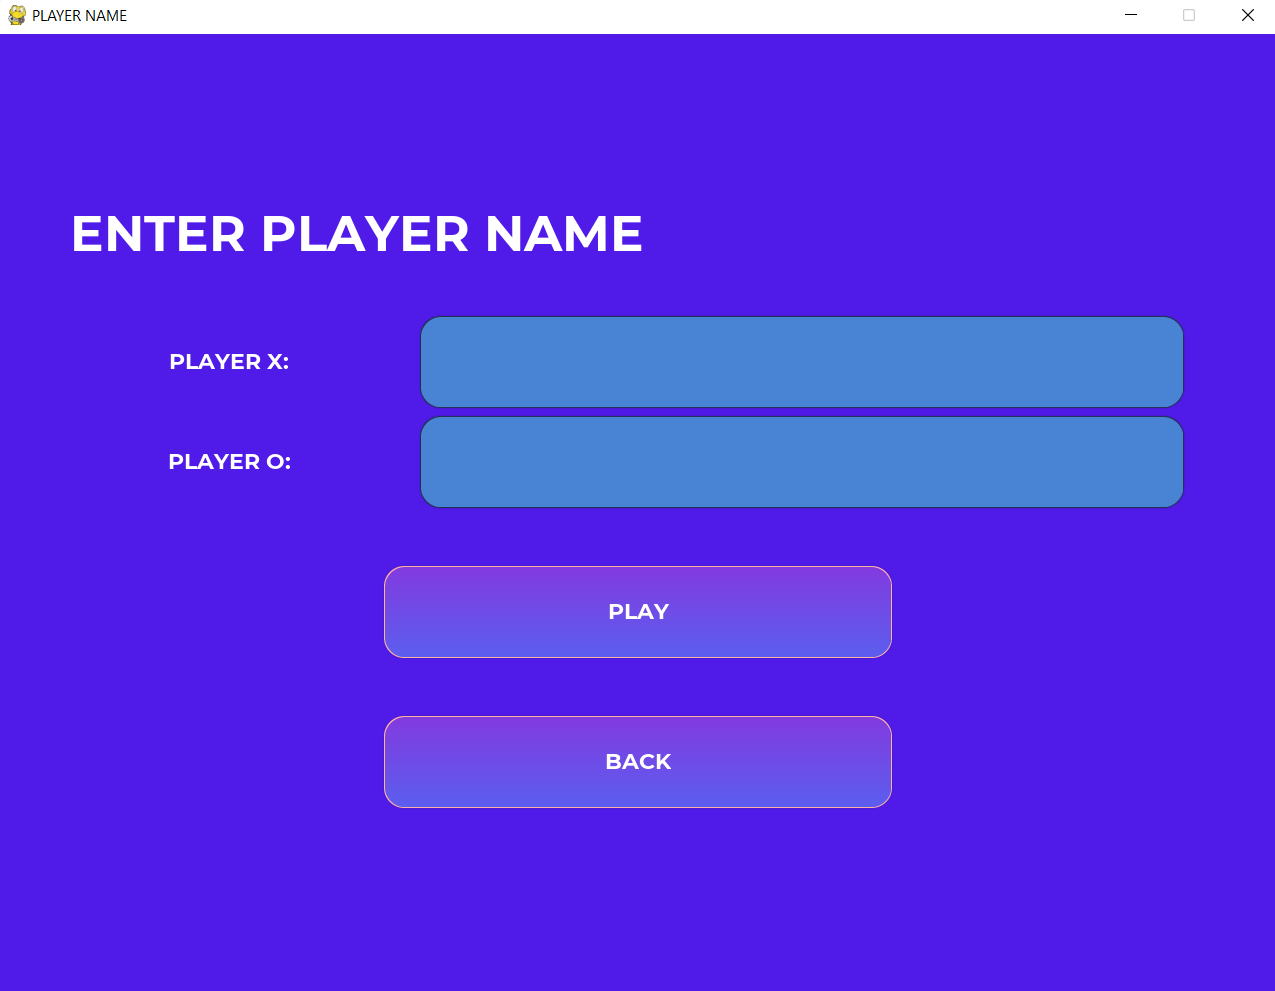
\includegraphics[scale=0.5]{images/playername.png}}
\caption{Màn hình đặt tên người chơi}
\end{figure}
\subsection{Màn hình game khi chơi}
Sau khi nhập tên 2 người chơi thành công và nhấn \verb|Play|, màn hình game khi chơi sẽ hiện ra như hình bên dưới. Ở đây ta lấy màn hình khi chơi một ván caro \(5\) quân với kích cỡ bàn cờ là \(16 \times 16\).
\begin{figure}[H]
\centering{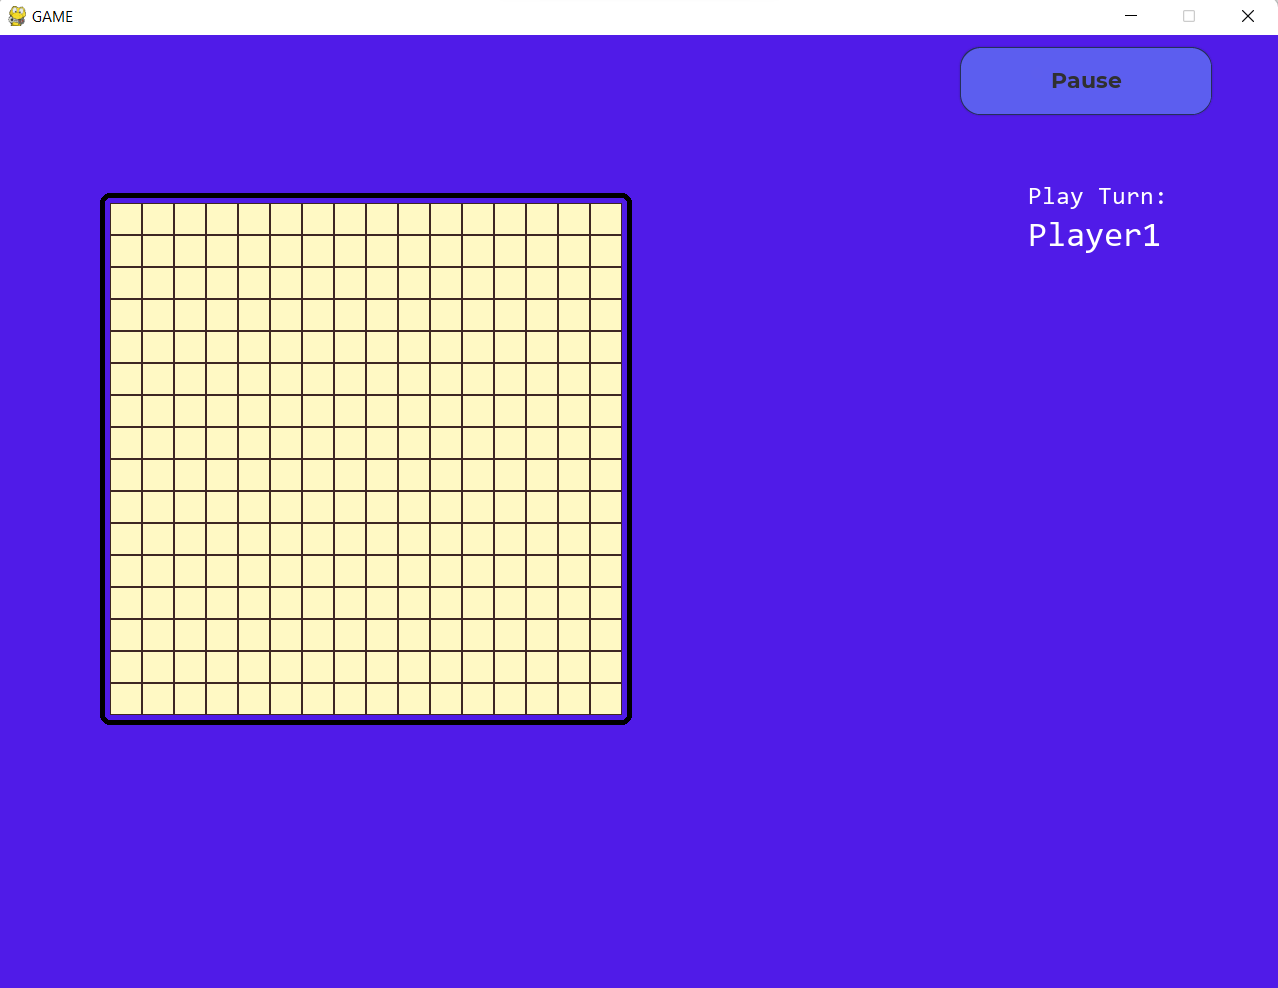
\includegraphics[scale=0.5]{images/playscreen.png}}
\caption{Màn hình game khi đang chơi}
\end{figure}
Khung \verb|Play Turn| trên màn hình ván game nhằm hiển thị tên người chơi ở mỗi lượt đánh:
\begin{figure}[H]
\centering{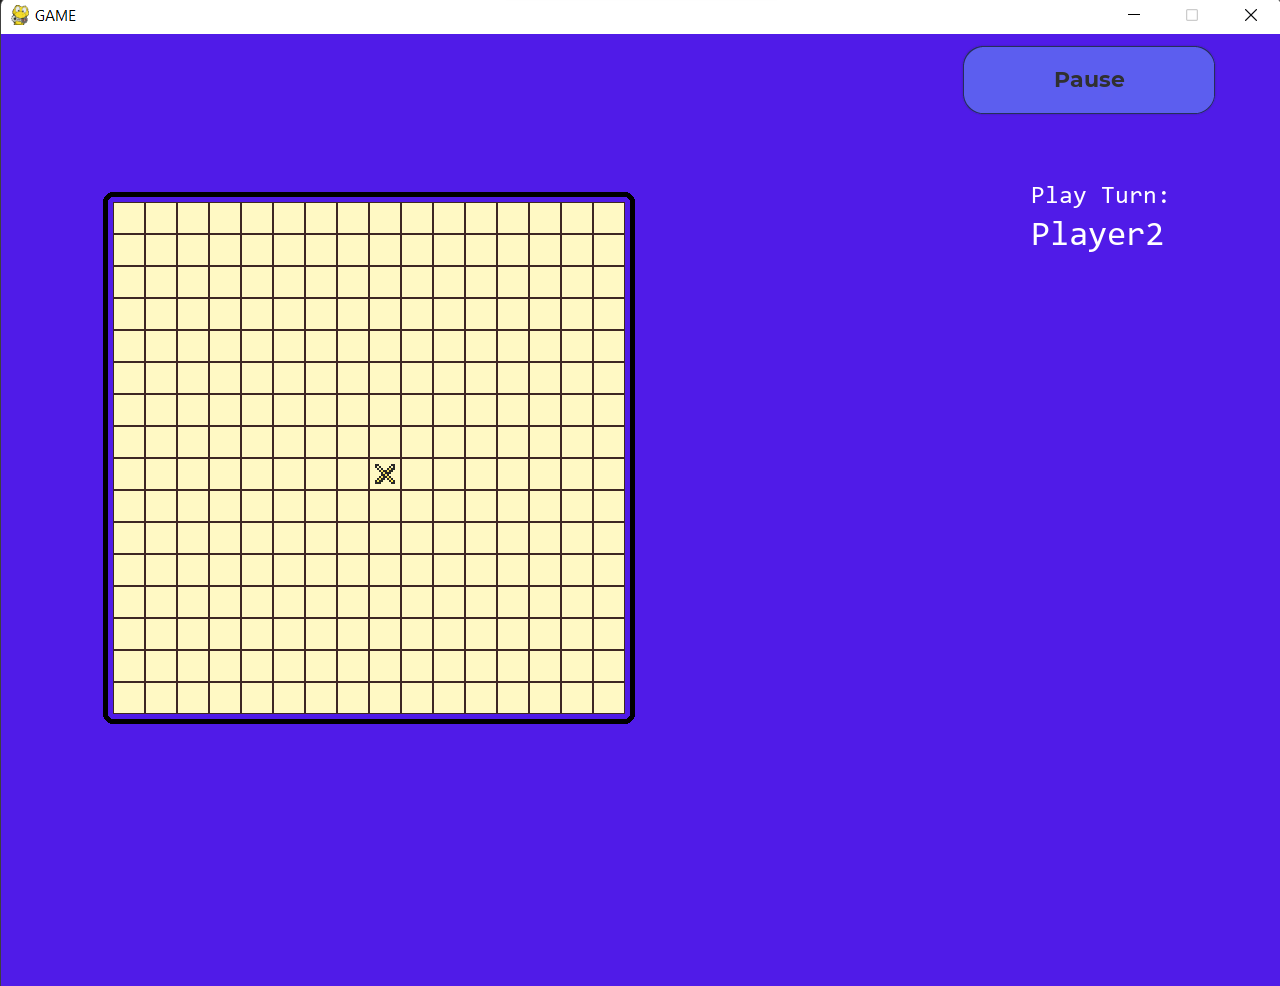
\includegraphics[scale=0.5]{images/player2.png}}
\caption{Màn hình game hiển thị tên người chơi thứ nhất}
\end{figure}
Sau khi người chơi đánh xong một ô cờ, khung đổi sang tên của người chơi còn lại cho lượt đánh kế tiếp:
\begin{figure}[H]
\centering{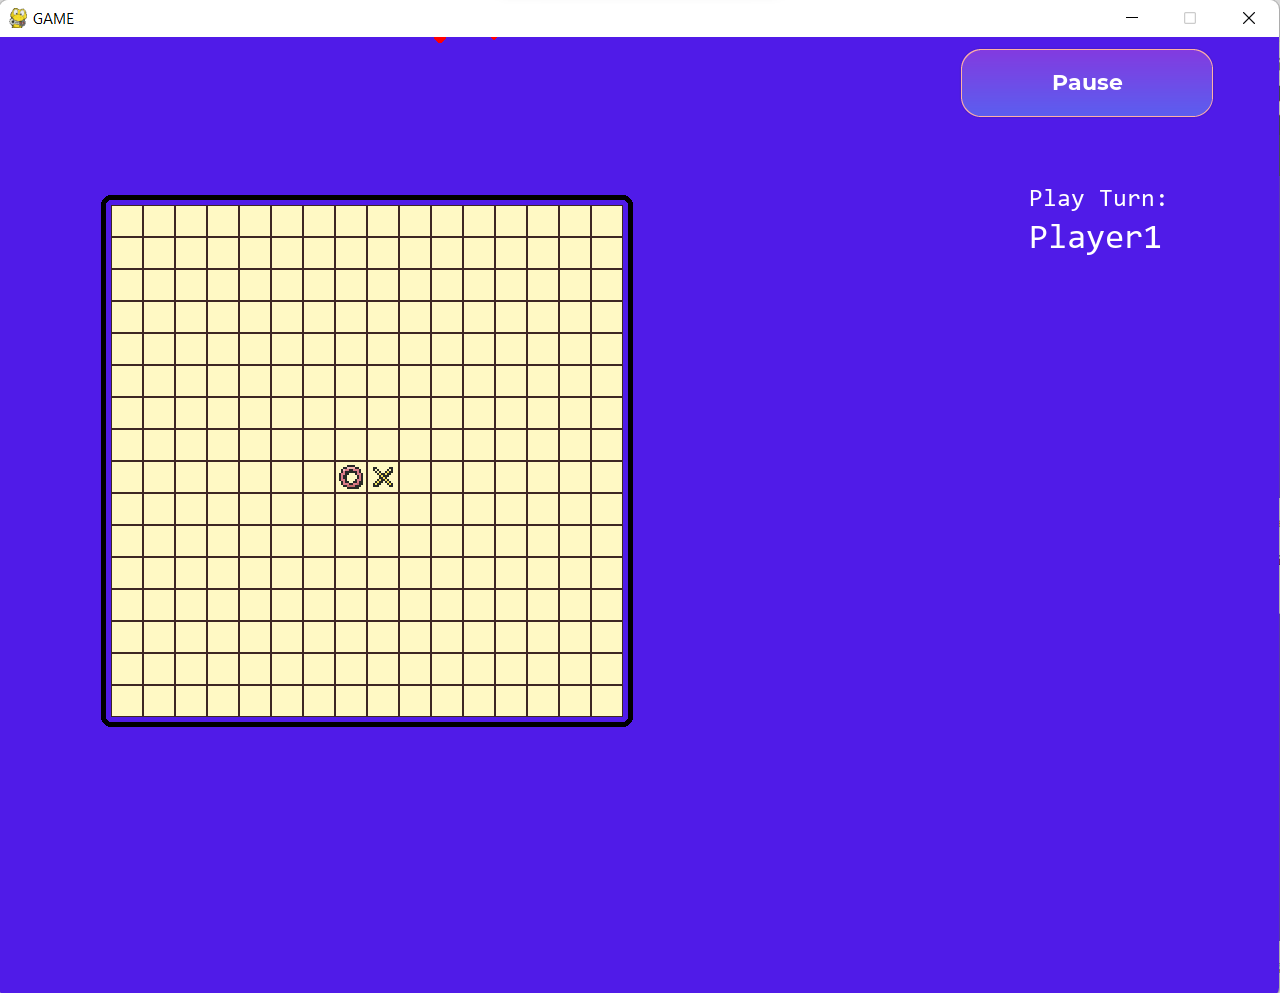
\includegraphics[scale=0.5]{images/player1.png}}
\caption{Màn hình game hiển thị tên người chơi thứ hai}
\end{figure}

Ở màn hình chơi ta có lựa chọn tạm dừng game (\verb|Pause|) để có thể tạm dừng ván đấu. Khi ta ấn vào nút \verb|Pause| ở góc phải trên của màn hình, một cửa sổ nhỏ hiện ra cho ta hai lựa chọn: lựa chọn bên trái là quay trở lại và tiếp tục ván đấu (nút \verb|Resume|), lựa chọn bên phải là quay lại màn hình khởi động (màn hình Menu), lưu ý khi ta quay lại Menu thì dữ liệu ván đấu hiện có sẽ được lưu lại. \\
Hình bên dưới đây là cửa sổ tạm dừng \verb|Pause|.
\begin{figure}[H]
  \centering{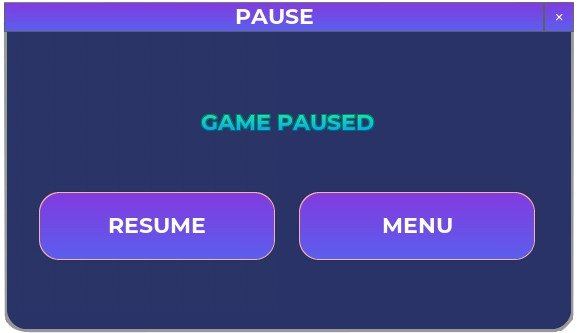
\includegraphics[scale=0.5]{images/pause.jpg}}
  \caption{Cửa sổ Pause}
\end{figure}
\subsection{Cửa sổ thông báo chiến thắng}
Sau khi 1 trong 2 người chơi tạo được một đường chéo, ngang hoặc dọc liên tiếp số con cờ caro (tương ứng với số quân cờ liên tiếp để thắng được chọn ở cửa sổ Setting), ngoài ra, những con cờ này không bị chặn ở 2 đầu thì cửa sổ thông báo tên người chơi chiến thắng sẽ hiện lên như hình bên dưới. Đồng thời, nhạc thông báo chiến thắng cũng được phát.
\begin{figure}[H]
  \centering{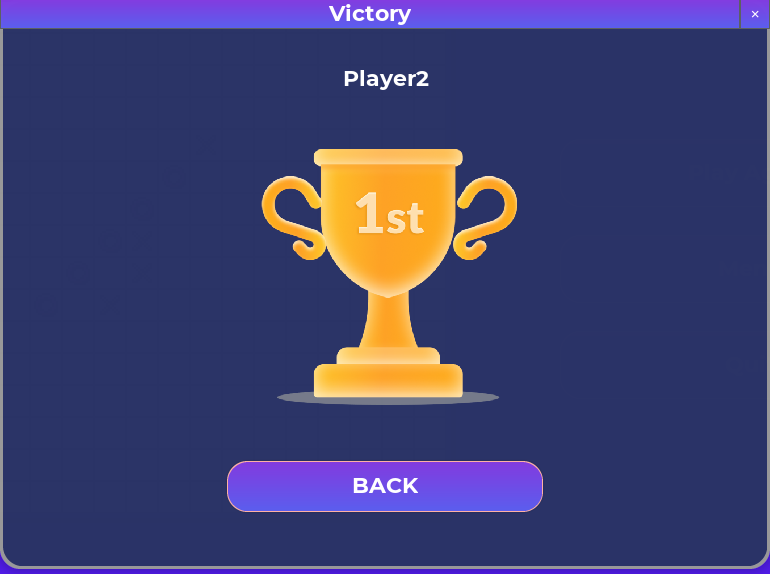
\includegraphics[scale=0.5]{images/win.png}}
  \caption{Cửa số Win}
\end{figure}
Người chơi nhấn nút \verb|Back| hoặc nút \verb|X| trên cùng bên phải của ô cửa sổ Win để quay lại màn hình game. Khi đó, màn hình game sẽ hiện thêm 3 chức năng cho người chơi lựa chọn như hình bên dưới.
\begin{figure}[H]
  \centering{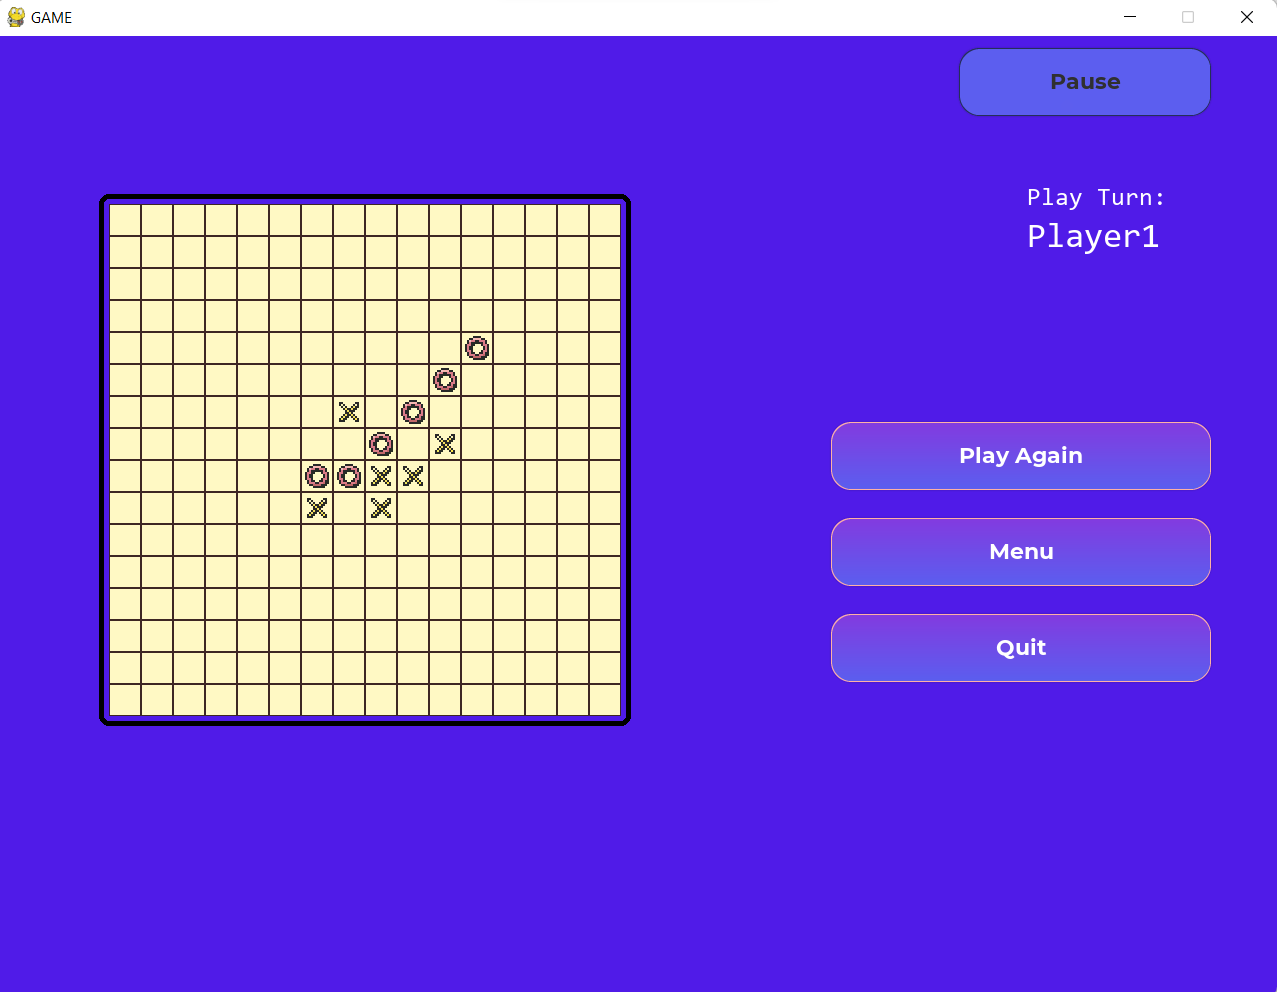
\includegraphics[scale=0.5]{images/afterwinscreen.png}}
  \caption{Màn hình game sau khi tắt cửa sổ Win}
\end{figure}
Khi người chơi chọn nút \verb|Play Again|, màn hình game sẽ khởi tạo ván game mới. Nút \verb|Menu| dùng để quay lại màn hình khởi động của game. Với nút \verb|Quit| khi được chọn, ô cửa sổ Quit sẽ hiện ra.
\subsection{Cửa sổ Quit}
Để mở ra ô cửa sổ Quit, người chơi có thể thực hiện một trong các thao tác sau: nhấn vào nút \verb|Quit| trên màn hình khởi động của game, nhấn nút \verb|X| trên cùng bên phải của màn hình game, hoặc nhấn nút \verb|Quit| trên màn hình game sau khi tắt ô cửa sổ Win. Khi đó, cửa sổ Quit sẽ hiện ra như hình bên dưới. Người chơi có thể thực hiện 2 chức năng trên ô cửa sổ này. Nhấn nút \verb|Exit| để thoát khỏi phần mềm game. Nhấn nút \verb|Keep Playing| hoặc nút \verb|X| ở trên cùng bên phải cửa sổ Quit để tắt ô cửa sổ Quit, tiếp tục thực hiện các thao tác trên màn hình game.
\begin{figure}[H]
\centering{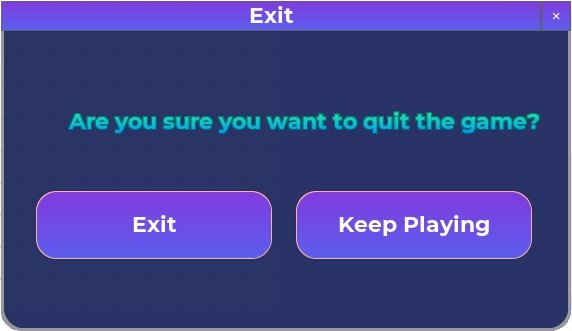
\includegraphics[scale=0.5]{images/quit.png}}
\caption{Cửa sổ Quit}
\end{figure}